\section{ビルド環境の検証}

これは外部ファイルから読み込まれたテキストです。
日本語のレンダリング、全角スペース（　）、
および記号（①、～）が正しく出力されるかテストします。

\begin{figure}[H]
    \centering
    
\includegraphics[width=0.5\textwidth]{figures/test_image.png}
    \caption{テスト用画像の読み込み}
    \label{fig:test_image1}
\end{figure}

\begin{figure}[H]
    \centering
    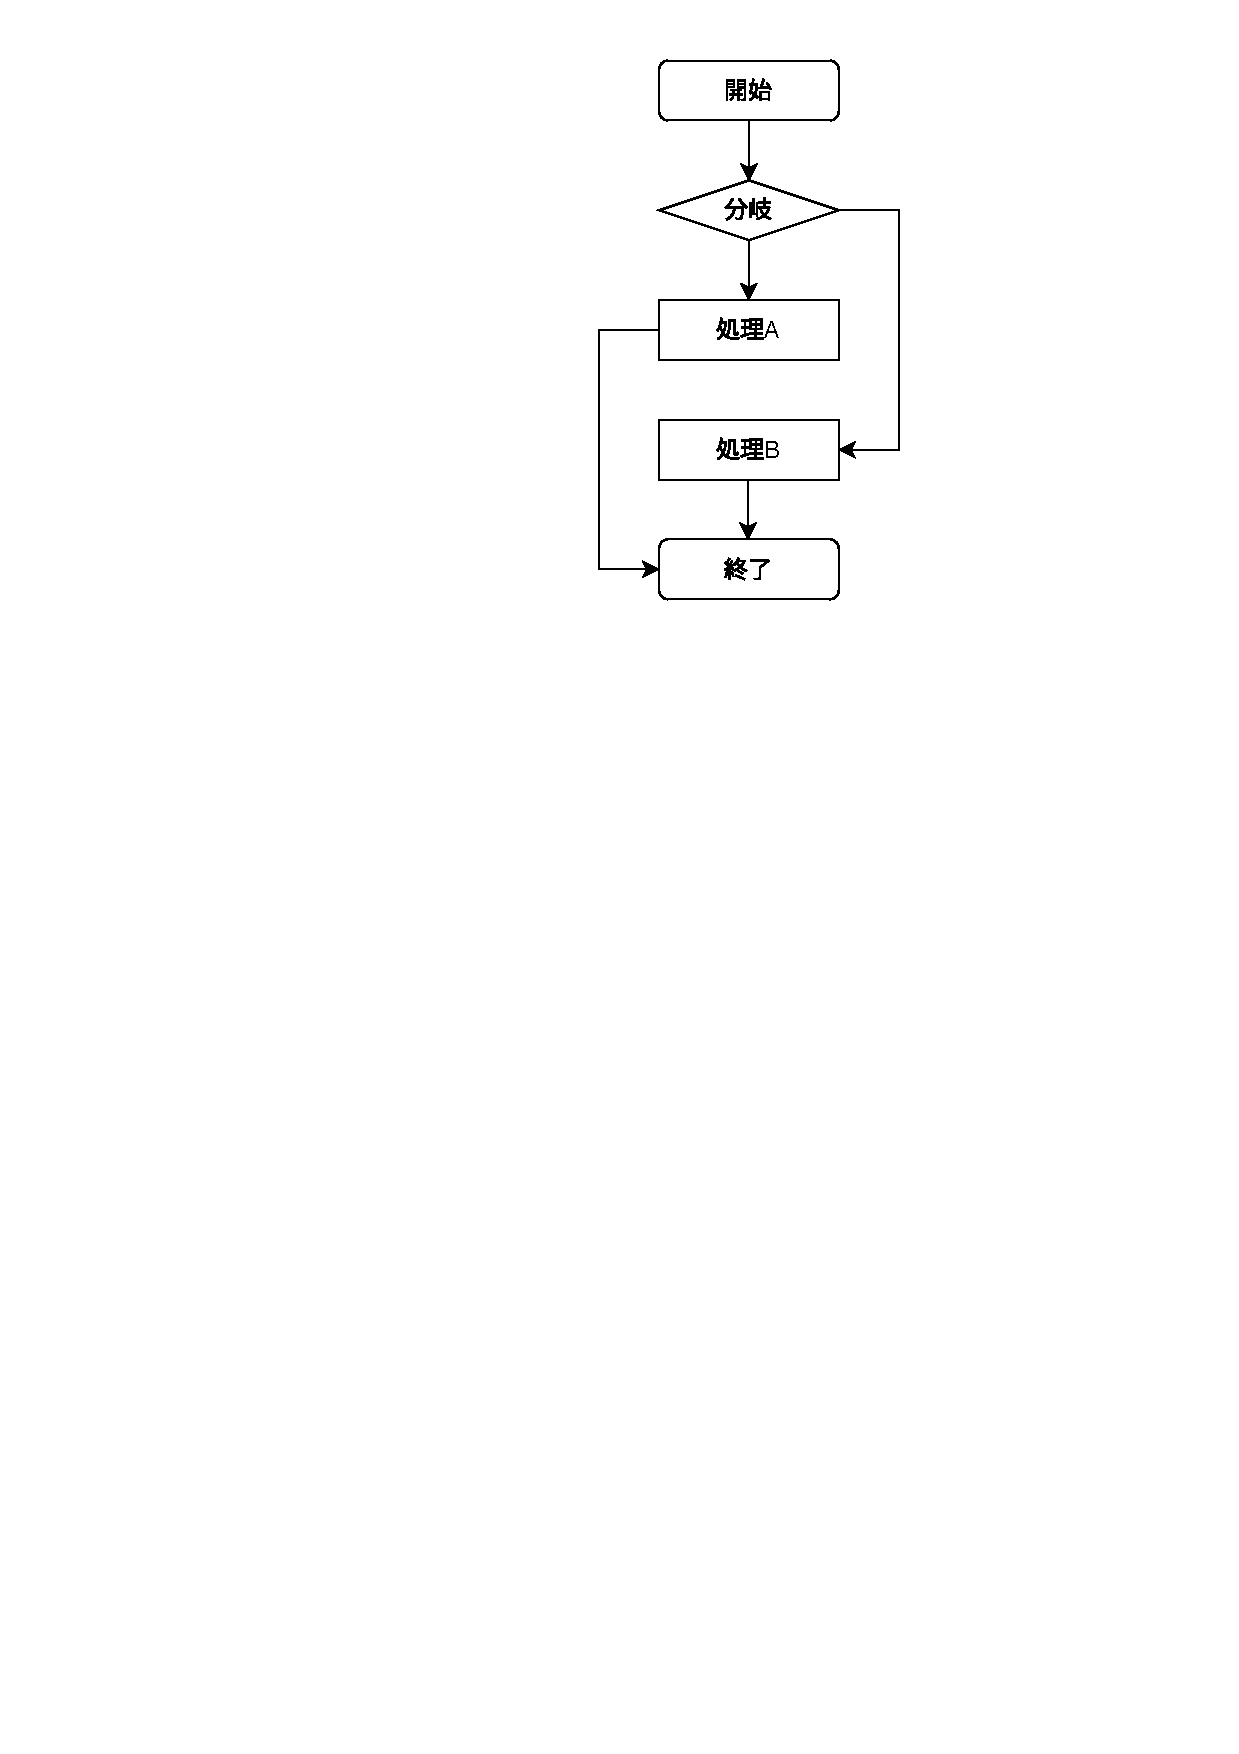
\includegraphics[width=0.5\textwidth]{figures/テスト用フロー図.pdf}
    \caption{テスト用画像の読み込み}
    \label{fig:test_image2}
\end{figure}

図\ref{fig:test_image1}および図\ref{fig:test_image2}は、
画像ディレクトリからの読み込みと相互参照のテストです。
複数回コンパイルが回っていれば、ここに正しい番号が入ります。
